\documentclass[12pt]{article}
\usepackage{tikz}
\usetikzlibrary{positioning}

\begin{document}
	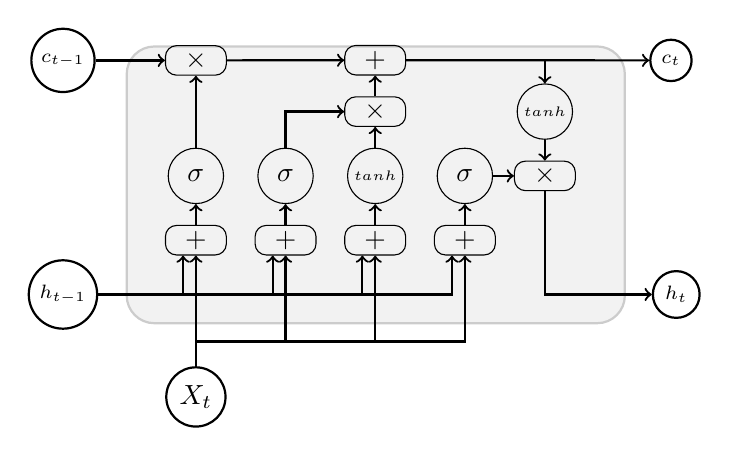
\begin{tikzpicture}[operation/.style={rectangle,draw,align=center, minimum width=2.2em, minimum height=.5em,inner sep=2pt,rounded corners=4}, links/.style={->, thick}]
	
		\draw[rounded corners=10,black!20!white, thick, fill=black!5!white ] (0,0) rectangle (18em,-10em);
		
		\node[operation] at (2.5em, -7em) (addition1) {$+$};
		\node[operation, right = 1em of addition1] (addition2) {$+$};
		\node[operation, right = 1em of addition2] (addition3) {$+$};
		\node[operation, right = 1em of addition3] (addition4) {$+$};
		
		
		\node[draw, circle, above = 0.75em of addition1, minimum size=20] (sigma1) {$\sigma$};
		\node[draw, circle, above = 0.75em of addition2, minimum size=20] (sigma2) {$\sigma$};
		\node[draw, circle, above = 0.75em of addition3, inner sep=1, minimum size=20] (tanh1) {\tiny $tanh$};
		\node[draw, circle, above = 0.75em of addition4, minimum size=20] (sigma3) {$\sigma$};
		
		
		\node[operation, above = 0.75em of tanh1] (times1) {$\times$};
		\node[operation, above = 0.75em of times1] (addition5) {$+$};
		
		\node[operation, right = 0.75em of sigma3] (times2) {$\times$};
		\node[draw, circle, above = 0.75em of times2, inner sep=1, minimum size=20] (tanh2) {\tiny $tanh$};
		
		\node[operation, above = 2.6em of sigma1] (times3) {$\times$}; 
		
		\node[circle, draw, thick, inner sep = 2.5, below = 4em of addition1] (input) {$X_t$};
		
		
		
		\node[circle, draw, thick, inner sep = 2.5, left = 2.5em of times3] (previouscellstate) {\scriptsize $c_{t-1}$} ;
		
		\node[circle, draw, thick, inner sep = 2.5, below = 6em of previouscellstate] (previoushiddenstate) {\scriptsize $h_{t-1}$} ;
		
			\node[circle, draw, thick, inner sep = 2.5, right = 20em of previoushiddenstate] (nexthiddenstate) {\scriptsize $h_{t}$} ;
		
		\node[circle, draw, thick, inner sep = 2.5, right = 20em of previouscellstate] (nextcellstate) {\scriptsize $c_{t}$} ;
		
		\draw[links] (previouscellstate) -- (times3);
		\draw[links] (addition5) -- (nextcellstate);
		
		\draw[links] (input) -- (addition1);
		\draw[links] (input) |- ++(3em,2em) -| (addition2);
		\draw[links] (input) |- ++(5em,2em) -| (addition3);
		\draw[links] (input) |- ++(7em,2em) -| (addition4);
		
		\draw[links] (previoushiddenstate) -|  (addition1.230);
		\draw[links] (previoushiddenstate) -|  (addition2.230);
		\draw[links] (previoushiddenstate) -|  (addition3.230);
		\draw[links] (previoushiddenstate) -|  (addition4.230);
		
		\draw[links] (times2) |- (nexthiddenstate);
		
		\draw[links] (addition1) -- (sigma1);
		\draw[links] (addition2) -- (sigma2);
		\draw[links] (addition3) -- (tanh1);
		\draw[links] (addition4) -- (sigma3);
		
		\draw[links] (tanh1) -- (times1);
		\draw[links] (times1) -- (addition5);
		\draw[links] (sigma2) |- (times1);
		
		\draw[links] (sigma1) -- (times3);
		
		\draw[links] (times3) -- (addition5);
		\draw[links] (addition5) -| (tanh2);
		\draw[links] (tanh2) -- (times2);		
		\draw[links] (sigma3) -- (times2);
	\end{tikzpicture}
\end{document}